\chapter{Planetbevægelse}\label{cha:Planet}
I dette kapitel skal vi undersøge klassisk bevægelse i stjernesystemer. Specifikt skal vi kigge på Keplers love og ud fra Lagrangemekanik undersøge, hvordan planeter, kometer og lignende bevæger sig omkring tungere objekter såsom stjerner. Vi vil tage udgangspunkt i det generelle tolegemeproblem, hvor to legemer påvirker hinanden med en indbyrdes centralkraft. Herefter vil vi kigge på det særlige tilfælde, hvor denne kraft er omvendt proportional med afstanden imellem de to legemer kvadreret, og til sidst sætter vi denne kraft til at være tyngdekraften. Til dette vil vi introducere keglesnit og vise, at bevægelserne der fremkommer kan beskrives ud fra de geometriske former, der fås ved at snitte en kegle på forskellige måder.


\section{Planetbaner og excentricitet}
Når objekter er i bevægelse om et centralt legeme, for eksempel en planet omkring en stjerne, kan deres baner generelt have tre forskellige former: Elliptiske, parabolske og hyperbolske. Formen af disse afhænger af banernes excentricitet $\epsilon$, som beskriver, hvor tæt banerne er på at være perfekt cirkelformede.

\subsection{Excentricitet fra keglesnit}
\begin{figure}[h!]
	\centering
	\begin{subfigure}{0.45\textwidth}
		\centering
		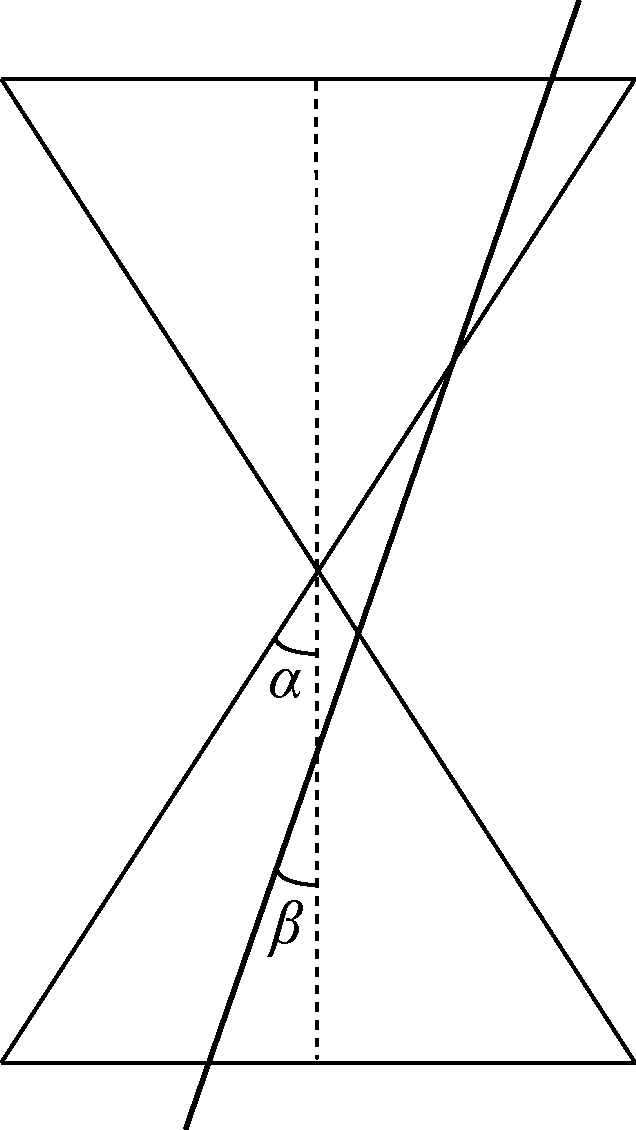
\includegraphics[width=0.55\textwidth]{Planetbevaegelse/KeglePlan.pdf}
		\caption{En dobbeltkegle med vinkel $\alpha$ til den horisontale akse (stiplet linje) skæres af et plan (breddere linje) med en vinkel $\beta$ til den vertikale akse.}
		\label{fig:KeglePlan}
	\end{subfigure}
	\hspace{5mm}
	\begin{subfigure}{0.45\textwidth}
		\centering
		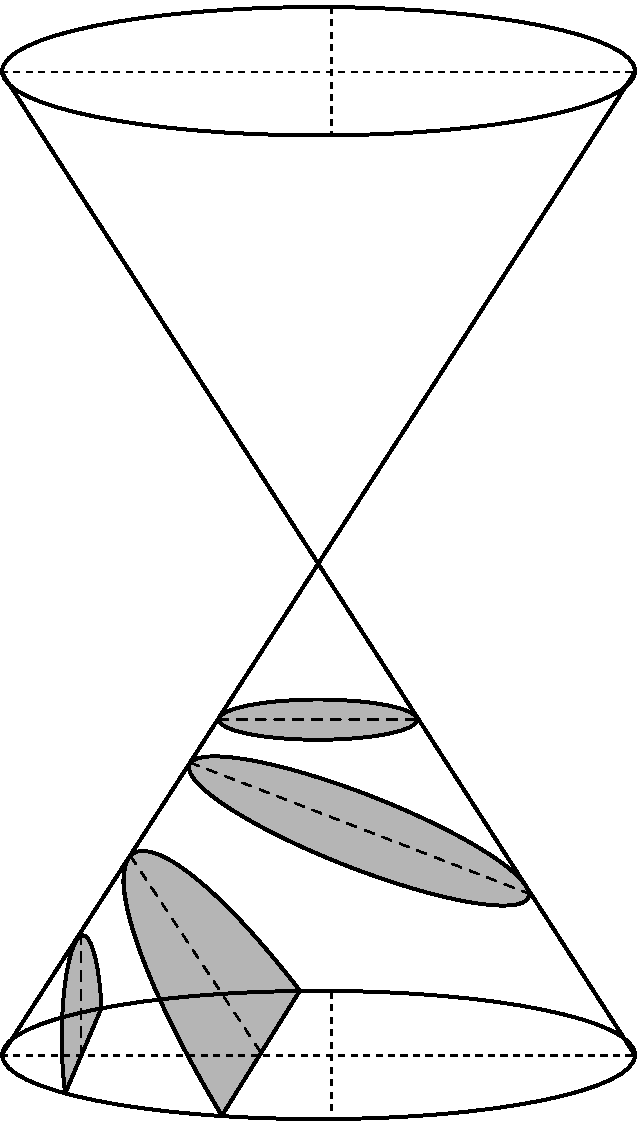
\includegraphics[width=0.55\textwidth]{Planetbevaegelse/KegleOrbit.pdf}
		\caption{Banerne fremkommer ved keglesnit med forskellige vinkler (fra øverst): Cirkel ($\epsilon = 0$), ellipse ($0 < \epsilon < 1$), parabel ($\epsilon = 1$) og hyperbel ($\epsilon > 1$).}
		\label{fig:KegleOrbit}
	\end{subfigure}
	\caption{En dobbeltkegle og dens keglesnit, som resulterer i forskellige planetbaner.}
\end{figure}

Ses på en dobbeltkegle dannet af en ret linje, der roterer omkring en fastlåst akse, og et plan der skærer denne kegle, figur \ref{fig:KeglePlan}, da kan excentriciteten af det keglesnit, der opstår, beskrives ved
\begin{align}
	\epsilon &\equiv \frac{\cos(\beta)}{\cos(\alpha)} \: .
\end{align}
Her betegner $\alpha$ og $\beta$ vinklen mellem den horisontale akse i keglen og henholdsvis keglesiden og planet. For $\alpha$ og $\beta$ skal det gælde, at $0<\alpha<\pi/2$, da keglen skal være en kegle og ikke blot en vertikal eller horisontal linje, og $0 \le \beta \le \pi/2$, da planet må være alt fra og med vertikalt til og med horisontalt.
Nogle af de keglesnit der fremkommer ved dette, kan ses på figur \ref{fig:KegleOrbit}, og de fremkommer på følgende måder:
\begin{itemize}
	\item \textbf{Elliptiske baner:} Idet planet skærer keglen i en vinkel større end keglens vinkel\footnote{Dette afsnit gør sig gældende så længe, at planet ikke skærer dobbeltkeglen i samlingspunktet mellem de to kegler, altså hvor de to kegles spidser mødes, da der så ville være tale om degenererede keglesnit.}, således at $\beta > \alpha$, vil elliptiske baner forekomme, da planet skærer begge sider af keglen, hvorfor banen er lukket. Excentriciteten af disse baner bliver derved $\epsilon < 1$. Cirkelbaner er et specialtilfælde af de elliptiske baner, hvor excentriciteten er $\epsilon = 0$.
	\item \textbf{Parabolske baner:} Når planet skærer keglen i en vinkel lig keglens vinkel, $\alpha = \beta$, opstår en parabolsk bane. Siden denne bane er parallel med keglesiden, vil denne være grænsen mellem lukkede og åbne baner. Excentriciteten af sådanne baner er $\epsilon = 1$.
	\item \textbf{Hyperbolske baner:} Tilbage er når planet skærer dobbeltkeglen i en vinkel mindre end keglens vinkel, så $\beta < \alpha$, hvorved der dannes en hyperbolsk bane, da planet kun skærer hver af keglerne i dobbeltkeglen ét sted, hvorfor der dannes en åben bane. Ud fra de givne vinkler er excentriciteten af en hyperbolsk bane givet ved $\epsilon > 1$.
\end{itemize}

\subsection{Fysisk definition af excentricitet}
\begin{figure}[h!]
	\centering
	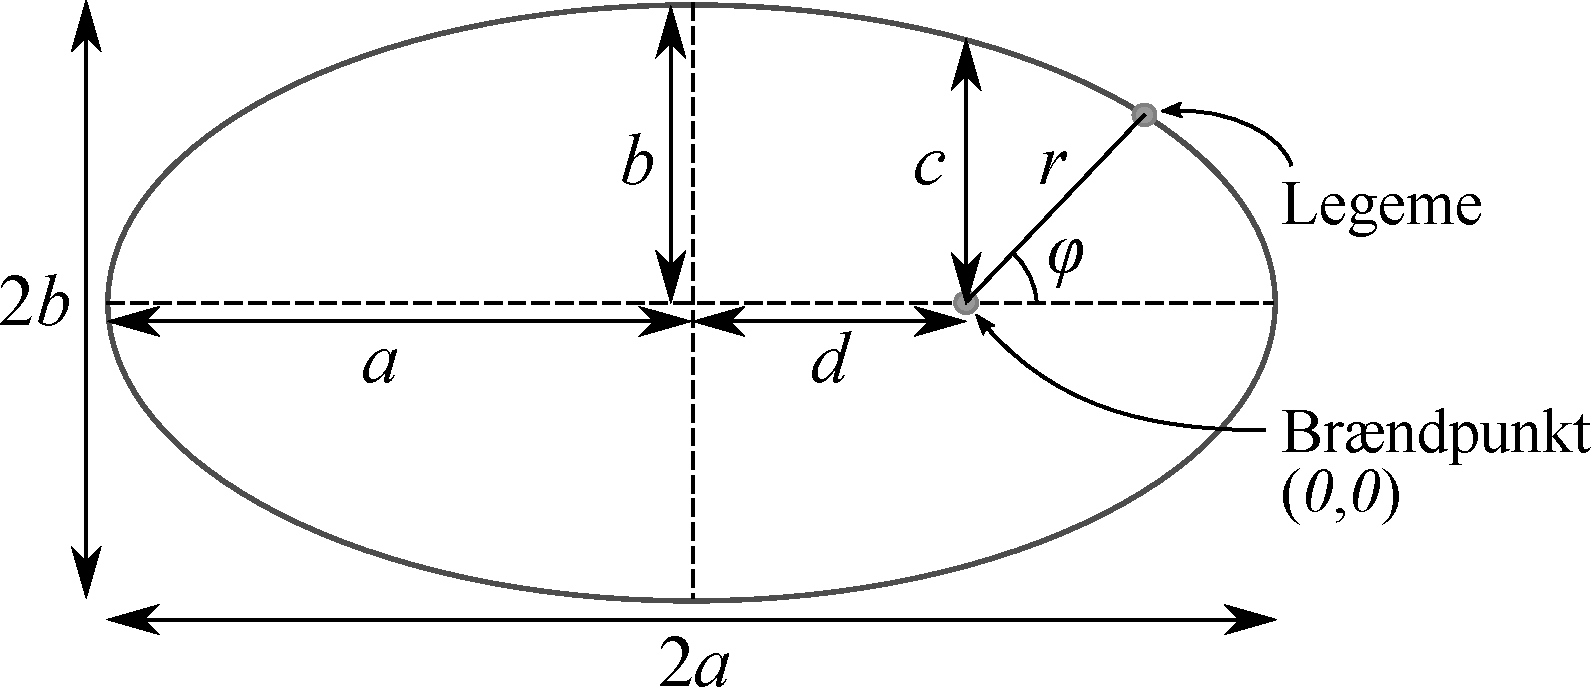
\includegraphics[scale=0.45]{Planetbevaegelse/Ellipse.pdf}
	\caption{Elliptisk bane hvor $a$ og $b$ betegner henholdsvis den halve storakse og den halve lilleakse, $d$ er forskydningen af brændpunktet fra ellipsens centrum, $c$ er afstanden af et linjestykke fra brændpunktet til punktet på ellipsen, hvor dette linjestykke er vinkelret på storaksen, og $r$ er afstanden fra brændpunktet til et virkårligt sted på ellipsen i en vinkel $\phi$. Ved udregninger antages brændpunktet at ligge i $(0,0)$.}
	\label{fig:Ellipse}
\end{figure}

Mens denne beskrivelse af excentricitet virker fint til matematisk at beskrive ellipser, parabler og hyperbler, da er den ikke specielt brugbar til beregning af excentriciteten af planetbaner, da man ikke har en kegle i rummet at gå ud fra. Af denne grund findes en anden og ækvivalent definition af excentricitet, som tager udgangspunkt i de parametre, som kan måles for en planetbane:
\begin{align}
	\epsilon &\equiv \frac{d}{a} \: .
\end{align}
Her er $a$ den halve storakse, og $d$ er afstanden fra et brændpunkt til centrum af banen, se figur \ref{fig:Ellipse}. \\
\noindent
Excentriciteten af en planetbane bruges til at beregne afstanden mellem to objekter, hvor det ene objekt befinder sig i bane om det andet i vilkårlig vinkel $\phi$, som angivet på figur \ref{fig:Ellipse}. Ligningen for banens radius, som funktion af vinklen af et objekt, ligning \eqref{eq:Ellipse_i_polaere_koordinater}, kan findes ved at konvertere formlerne for en elliptisk bane med nulpunkt i et brændpunkt, ligning \eqref{eq:Ellipse_i_kartesiske_koordinater}, en parabolsk bane, ligning \eqref{eq:Parabel_i_kartesiske_koordinater}, og en hyperbolsk bane, ligning \eqref{eq:Hyperbel_i_kartesiske_koordinater}, fra kartesiske koordinater:
\begin{align}
	1 &= \frac{(x+d)^2}{a^2} + \frac{y^2}{b^2} \label{eq:Ellipse_i_kartesiske_koordinater} \\
	y^2 &= c^2 - 2cx \label{eq:Parabel_i_kartesiske_koordinater} \\
	1 &= \frac{(x-\delta)^2}{\Gamma^2}-\frac{y^2}{\eta^2} \: , \label{eq:Hyperbel_i_kartesiske_koordinater}
\end{align}
hvor $a$, $b$ og $d$ er givet ved følgende formler:
\begin{equation} \label{eq:Planetbevaegelse_a_b_og_d}
	\begin{aligned}
		a &= \frac{c}{1-\epsilon^2} \\
		b &= \frac{c}{\sqrt{1-\epsilon^2}} \\
		d &= a\epsilon \: ,
	\end{aligned}
\end{equation}
og $\Gamma$, $\delta$, $\eta$ og $c$ er konstanter, til polære koordinater. Dette viser sig at give én og samme ligning
\begin{align} \label{eq:Ellipse_i_polaere_koordinater}
	r(\phi) &= \frac{c}{1+\epsilon\cos(\phi)} \: ,
\end{align}
hvilken vi senere viser at planetbaner opfylder.

\section{Tolegemeproblemet}
Til at udlede Keplers love, er det relevant at kende lidt mere til det problem vi arbejder med. Vi starter med et mere generelt tilfælde, end det vi vil undersøge, nemlig det generelle tolegemeproblem. Det er et system hvor følgende er opfyldt: Systemet skal indeholde præcis to legemer, der påvirker hinanden med en indbyrdes central, konservativ kraft. At kraften er central betyder, at den udelukkende afhænger af afstanden mellem de to legemer. At den er konservativ betyder, at arbejdet den udfører på et af legemerne, ikke afhænger af vejen taget, men kun af start- og slutpunkt for vejen.\\
Vi kigger på to legemer med massen $m_1$ og $m_2$, der betragtes som punktpartikler, se figur \ref{fig:planet_relativ}. Vi opskriver først systemet, som et inertialsystem, det vil sige et system, der bevæger sig med konstant hastighed i forhold til alle andre inertialsystemer. Dette system kan betragtes som værende i hvile, og det må ikke være roterende. I et inertialsystem har hvert legeme en vektor, der går fra origo og ud til legemet, henholdsvis $\subv{r}{1}$ og $\subv{r}{2}$. Legemerne påvirkes af en fælles tiltrækningskraft, henholdsvis $\subv{F}{21}$ og $\subv{F}{12}$, som antages at være konservativ og central. Da kræfterne er konservative, kan de udledes fra en potentiel energi $V(\subv{r}{1},\subv{r}{2})$. Vi vil senere sætte denne kraft til at være en gravitations kraft af størrelsen, $Gm_1m_2/|\subv{r}{1}-\subv{r}{2}|^2$, med tilhørende potentiel energi
\begin{align}
	V(\subv{r}{1},\subv{r}{2}) = -\frac{Gm_1m_2}{|\subv{r}{1}-\subv{r}{2}|}.
\end{align}
Bemærk her, at den potentielle energi kun afhænger af afstanden mellem legemerne, og ikke de individuelle vektorer. Dette er hvad det vil sige, at kraften er central, og det betyder også, at den potentielle energi ikke afhænger af hvilket inertialsystem, vi vælger. Potentielle energier, med denne egenskab, kaldes translationelt invariante. Det er altså lige meget for kraften og den potentielle energi, hvor origo ligger. \\
%
Der gælder derved nærmere, at $V(\subv{r}{1},\subv{r}{2}) = V(|\subv{r}{1}-\subv{r}{2}|)$, og det giver mening at introducere en ny vektor, $\v{r}$, som vi kalder den relative position:
\begin{align}
	\v{r} = \subv{r}{1}-\subv{r}{2}.
\end{align}
Afstanden imellem de to legemer, $r$, er således størrelsen af vektoren $\v{r}$, og $V=V(r)$. \\ \\
% Sæt figur op
%
\begin{figure}[h!]
\centering
	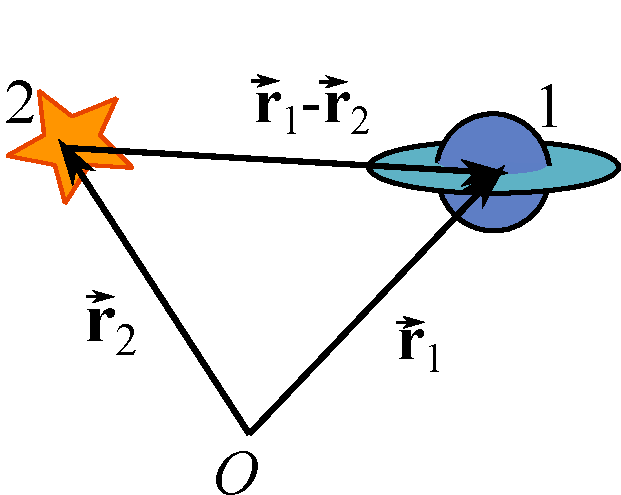
\includegraphics[width = 0.4\textwidth]{Planetbevaegelse/relativkoordinat_planet.pdf}
	\caption{Illustrerer vektorer $\v{r}_1$ og $\v{r}_2$ fra origo til hver af de to legemer, samt den relative positionsvektor $\v{r} = \v{r}_1 - \v{r}_2$ af legeme 1 i forhold til legeme 2.}
	\label{fig:planet_relativ}
\end{figure}
Nu kan problemets Lagrangefunktion opskrives:
\begin{equation}
\begin{aligned}
	L &= \frac{1}{2} m_1 \dt{\v r}_1^2 + \frac{1}{2} m_2 \dt{\v{r}}_2^2 - V(r) \\
	&= \frac{1}{2} m_1 \dt{\v{r}}_1^2 + \frac{1}{2} m_2 \dt{\v{r}}_2^2 + \frac{Gm_1m_2}{r}.
\end{aligned}
\end{equation}
Dette kunne også være opskrevet ud fra Newtons love, men i dette tilfælde holder vi os til vores nyligt lærte Lagrangemekanik.


\section{Massemidtpunkt, relative koordinater og reduceret masse}
Vi skal vælge hvilke generaliserede koordinater, vi vil opskrive og løse systemet i. Indtil videre har vi bare opskrevet problemet i et almindeligt inertialsystem med kartesiske koordinater og et vilkårligt nulpunkt. \\
%
Dog lægger systemet tydeligvis op til at man benytter et relativ koordinat, $\v{r}$, som en af vores generaliserede koordinater. Da systemet er centralt og kun involverer to legemer og kræfter, der følger en lige linje, behøver vi ikke mere end et 3-dimensionelt koordinat til hvert legeme\footnote{de oprindelige koordinater er $\subv{r}{1}$ og $\subv{r}{2}$}. Så indtil videre skal der bruges et koordinat mere, for at vi har lige så mange koordinater, som forventede frihedsgrader. Her vælges et koordinat, kaldet massemidtpunktet, eller "centre of mass coordinate"\;(med endepunkt CM), som betegnes $\v{R}$. Den er defineret som
\begin{align}\label{CM}
	\v{R} &= \frac{m_1 \subv{r}{1} + m_2 \subv{r}{2}}{m_1 + m_2} = \frac{m_1 \subv{r}{1} + m_2 \subv{r}{2}}{M} \, ,
\end{align}
hvor $M$ betegner den totale masse for systemet: $M = m_1 + m_2$. Da $\v{R}$ involverer en sum af de vægtede vektorer, viser det sig, at massemidtpunktet ligger på linjen mellem de to legemer, dannet af $\subv{r}{1} - \subv{r}{2}$. \\

%Figur 
%
\begin{figure}[h!]
\centering
	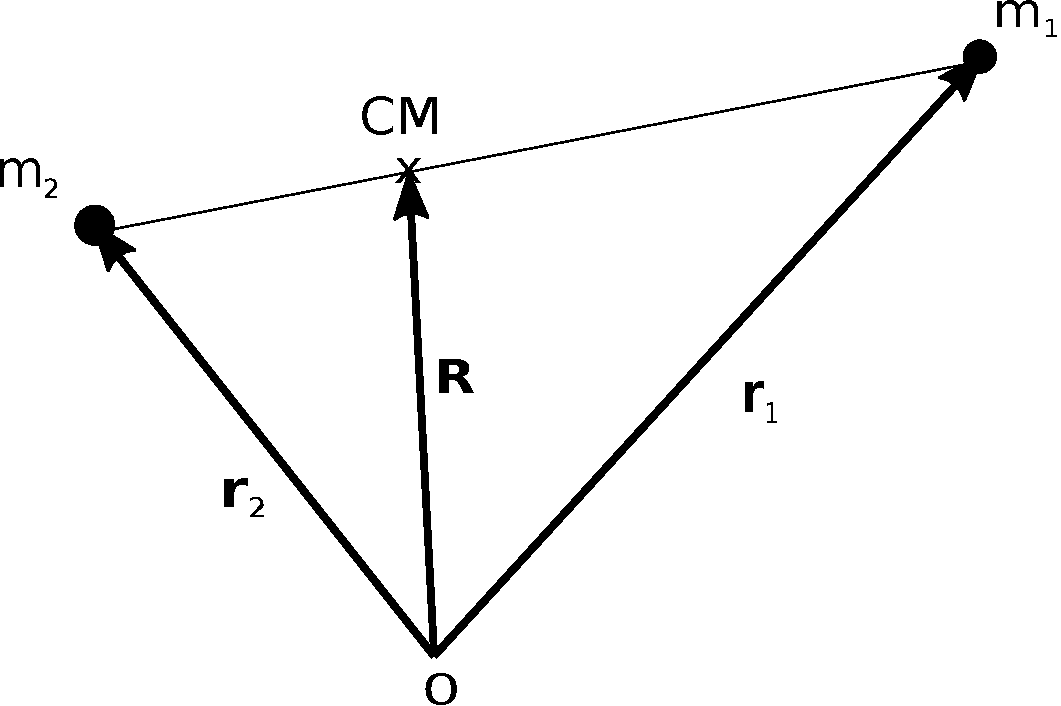
\includegraphics[width = 0.4\textwidth]{Planetbevaegelse/figur_CM.pdf}
	\caption{Massemidtpunktet for de to legemer ligger ved $\v{R} = (m_1 \v{r}_1 + m_2 \v{r}_2)/M$ på linjen mellem de to legemer.}
\end{figure}
Den totale impuls, $\v{P}$, for systemet er den samme, som den totale masse lagt til ændringsraten for $\v{R}$ i tiden:
\begin{align}
	\v{P} &= \dif{t}{} \left( m_1 \subv{r}{1} + m_2 \subv{r}{2} \right) = M \dt{\v{R}} .
\end{align}
Den totale impuls for systemet er konstant, da systemet ikke påvirkes af udefrakommende kræfter. Derfor må $\dt{\v{R}}$ være konstant, og der findes således et inertialsystem hvor $\dt{\v{R}}=\v{0}$ (inertialsystemer er systemer, der ikke accelererer). \\ \\
%
%
For at kunne introducere $\v{r}$ og $\v{R}$ som generaliserede koordinater i Lagrangefunktionen skal den kinetiske og potentielle energi omskrives til at være afhængig af dem, i stedet for de gamle koordinater. Vi ved allerede, at den potentielle energi let kan skrives, som afhængende kun af den relative afstand $r$. For den kinetiske energi skal vi først omskrive $\subv{r}{1}$ og $\subv{r}{2}$ til at afhænge af vores generaliserede koordinater. Fra definitionen af $\v{R}$ i ligning~\eqref{CM}, kan $\subv{r}{1}$ isoleres, og ved introduktion af definitionen af $\v{r}$ fås:
\begin{align}\label{Eq:r1}
	\subv{r}{1} = \v{R} + \frac{m_2}{M}\v{r}.
\end{align}
Det samme kan gøres med $\subv{r}{2}$, hvor der fås:
\begin{align}\label{Eq:r2}
	\subv{r}{2} = \v{R} - \frac{m_1}{M} \v{r}.
\end{align}
Den kinetiske energi bliver så:
\begin{equation}
\begin{aligned}
	K &= \frac{1}{2}(m_1 \dt{\v r}_1^2 + m_2 \dt{\v r}_2^2 ) \\
	  &=\frac{1}{2} \left(m_1 \left[\dt{\v{R}} + \frac{m_2}{M}\dt{\v{r}} \right]^2 + m_2 \left[\dt{\v{R}} - \frac{m_1}{M} \dt{\v{r}}\right] ^2 \right) \\
	  &= \frac{1}{2} \left( M \dt{\v{R}}^2 + \frac{m_1m_2}{M}\dt{\v{r}}^2\right),
\end{aligned}
\end{equation}
som reduceres yderligere til 
\begin{align}
	K = \frac{1}{2} M \dt{\v{R}}^2 + \frac{1}{2} \mu \dt{\v{r}}^2 \, ,
\end{align}
ved introduktion af en såkaldt "reduceret masse"\;$\mu$. Parameteren $\mu = \frac{m_1m_2}{M}$ har enheder af masse. \\
%
I de generaliserede koordinater er den kinetiske energi det samme, som en traditionel kinetisk energi for to "fiktive"\;partikler, en med massen $M$, der bevæger sig med samme hastighed som CM, og en med masse $\mu$, der bevæger sig med samme hastighed, som den relative position $\v{r}$. Derfor kan den samlede Lagrangefunktion splittes op i to dele, en for den relative bevægelse, og en for CM-bevægelsen:
\begin{equation}
\begin{aligned}
	L = K - V &= \frac{1}{2} M \dt{\v{R}}^2 + \left( \frac{1}{2}\mu \dt{\v{r}}^2 - V(\v r)\right) \\
	&= L_\text{CM} + L_\text{rel}.
\end{aligned}
\end{equation}
Derved kan de to koordinater løses som to separate problemer.
%
%
\section{Bevægelsesligningerne}
Ud fra den opskrevne Lagrangefunktion kan bevægelsesligningerne for systemet findes. Fra hovedemnet om Lagrangemekanik har vi Euler-Lagrange relationerne, ligning~\eqref{Euler-Lagrange}. Ved at benytte dem fås først bevægelsesligningerne for $\v{R}$ (bemærk her at $\v{R}$ teknisk set er en tre-dimensionel vektor, så der er tale om tre ligninger, for $X$, $Y$ og $Z$, som ellers er ens\footnote{Med ens menes der, at alle operationer vi benytter påvirker de tre koordinatligninger ens.}). Da Lagrangefunktionen ikke direkte afhænger af $\v{R}$ giver Euler-Lagrangeligningen i forhold til koordinatet $\v{R}$ at:
\begin{align}
	M\ddt{\v{R}} = \v{0},
\end{align}
som betyder, at $\dt{\v{R}}$ er konstant. Dette er allerede forklaret med, at den totale impuls for systemet er bevaret. Det kan også forklares ud fra, at Lagrangefunktionen er uafhængig af $\v{R}$, hvorfor der er tale om et negligibelt koordinat. Nærmere opfører $L_\text{CM}$ sig som en Lagrangefunktion for en fri partikel, med masse $M$ og position $\v{R}$. At det er et negligibelt koordinat betyder i sidste ende, at vores system nødvendigvis kun har en enkelt frihedsgrad, fremfor de to, som var forventet. \\ \\
%
%
Hvis Euler-Lagrangerelationen anvendes med hensyn til den 2. koordinat, $\v{r}$, fås:
\begin{align}
	\mu \ddt{\v{r}} &= - \grad{V(\v r)} = - \xyz{\partial V / \partial x}{\partial V / \partial y}{\partial V / \partial z} = \subv{F}{res}.
\end{align}
At gradienten af den samlede potentielle energi på et af legemerne, $\grad{V}$, er lig den resulterende kraft på legemet op til et fortegn, blev kort nævnt i mekanikkapitlet, men skyldes udelukkende, at vi kun arbejder med konservative kræfter. \\ \\
%
%
For at få bevægelsesen for det relative koordinat skal vi bare løse Newtons 2. lov for en enkelt partikel med reduceret masse $\mu$ og position $\v{r}$, i et potentiale $V(\v r)$.
%
%
\subsection*{Massemidtpunktsreferencesystemet}
Vi kan vælge et inertialsystem hvori $\dt{\v{R}} = \v{0}$, netop fordi $\dt{\v{R}}$ er konstant. Her vil den totale impuls for systemet være nul, og $L_\text{CM} = 0$. Derved bliver vores Lagrangefunktion
\begin{align}
	L = L_\text{rel} = \frac{1}{2} \mu \dt{\v{r}}^2 - V(\v r).
\end{align}
Problemet er reduceret til et etlegemeproblem, hvilket også var forventet, siden $\v{R}$ var et overflødig koordinat. \\ \\ % Lav en figur der viser bevægelsen i vores referencesystem

\subsection{Bevaring af impulsmoment}
Da der ikke er udefrakommende kræfter på systemet, må det, udover at betyde at totalimpulsen er bevaret, også betyde, at det totale impulsmoment (\textit{angular momentum}) også er bevaret. Det totale impulsmoment vil, ud fra de to oprindelige koordinater $\subv{r}{1}$ og $\subv{r}{2}$, være summen af de to legemers impulsmoment:
\begin{align}
	\v{L} &= \subv{r}{1} \times \subv{p}{1} + \subv{r}{2} \times \subv{p}{2} = \v r_1 \times m_1\dt{\v r}_1+\v r_2 \times m_2\dt{\v r}_2 \: .
\end{align}
Der benyttes her symbolet $\v{L} = \v{\ell}_1 + \v{\ell}_2$ for det totale impulsmoment, fordi man med ved brug af et stort bogstav indikerer, at der er tale om en sum af samme fysiske størrelse for flere legemer. I CM-referencesystemet, hvor origo er valgt til $\v{R} = \v 0$, fås specifikt fra ligningerne~\eqref{Eq:r1} og \eqref{Eq:r2} at:
\begin{align}
	\subv{r}{1} &= \frac{m_2}{M}\v{r} \\
	\subv{r}{2} &= -\frac{m_1}{M}\v{r}.
\end{align}
Derved fås, at det totale impulsmoment bliver:
\begin{equation}
\begin{aligned}
	\v{L} &= \frac{m_1 m_2}{M} \v{r} \times \frac{m_2}{M} \dt{\v{r}} - \frac{m_2 m_1}{M} \v{r} \times \left(-\frac{m_1}{M}\right) \dt{\v{r}} \\
	&= \frac{m_1m_2}{M^2}\left(m_2\v{r} \times \dt{\v{r}} + m_1 \v{r} \times \dt{\v{r}}\right) \\
	&= \v{r} \times \mu \dt{\v{r}}.
\end{aligned}
\end{equation}
hvor $m_1m_2/M$ er erstattet med den reducerede masse $\mu$. Herved ser vi også, at det totale impulsmoment for systemet i CM systemet svarer til det ækvivalente impulsmoment for en enkelt partikel med massen $\mu$ og positionen $\v{r}$. Da det totale impulsmoment er bevaret, må vektoren $\v{r} \times \dt{\v{r}}$ være konstant i både størrelse og retning. Dette betyder, at  de to vektorer beholdes indenfor et låst plan (2 dimensioner), som vi kan vælge som $xy$-planen. Derved har vi, udover at reducere tolegemeproblemet til et ækvivalent etlegemeproblem, desuden reduceret problemet fra et i 3 dimensioner til 2 dimensioner. Grunden til at vi tidligere har behandlet Lagrangefunktionen og tilhørende, som være en-dimensionel med hensyn til $\v{r}$, skyldes at alle operationer, vi har foretaget, på $\v{r}$, foretages ækvivalent på alle 3 rumlige dimensioner, og derved let kan overføres tilbage til et 3-dimensionelt system. \\
%
\subsection{De to bevægelsesligninger}
Vi har reduceret det oprindelige problem til kun at afhænge af en vektor $\v{r}$, og vi har reduceret $\v{r}$ til at være to-dimensionel. Dette betyder, at vi formentlig skal bruge to rumlige koordinater til, at beskrive problemets bevægelse fuldstændigt, hvor vi for eksempel kunne anvende $x,y$-koordinater. Da vi har med en bevægelse, der formentligt er cirkulær eller elliptisk, at gøre, er det nok smartere at vælge vores koordinater til at være polære, det vil sige en radius, $r$, (bemærk at denne er en skalar og ikke en vektor), og en vinkel, $\phi$. Dette giver en Lagrangefunktion på formen
\begin{align}
	L = \frac{1}{2}\mu\left(\dt{r}^2 + r^2 \dt{\phi}^2\right) - V(r).
\end{align}
Da Lagrangefunktionen ikke direkte afhænger af $\phi$ (udifferentieret), vil $\pdif{\phi}{L} = 0$, og derved giver Euler-Lagrangeligningen, at $\dif{t}{} \pdif{\dt{\phi}}{L} = 0$. Da må
\begin{align}
	\pdif{\dt{\phi}}{L} = \mu r^2 \dt{\phi} = \text{konstant} = \ell .
\end{align}
At konstanten her kaldes $\ell $ skyldes specifikt, at for polære koordinater (faktisk cylindriske koordinater), med et impulsmoment udelukkende i $z$-retningen, vil størrelsen af impulsmomentet $\ell $ for et legeme, være givet ved $m r^2 \dt{\phi}$. I dette tilfælde er vores problem netop ækvivalent med problemet for et enkelt legeme, hvor massen er givet ved $\mu$. \\
%
Da Euler-Lagrangeligningen for $\phi$ giver, at $\pdif{\phi}{L} = 0$, må $\phi$ være et negligibelt koordinat, og hele problemet burde altså kunne beskrives ud fra det ene koordinat $r(t)$, som et endimensionelt problem.\footnote{Det er nu endimensionelt netop fordi $r$ ikke er en vektor, men en skalar.} \\
%
Euler-Lagrangeligningen for det radielle komponent $r$ bliver
\begin{align}
	\pdif{r}{L} = \dif{t}{} \pdif{\dt{r}}{L}
\end{align}
og således
\begin{align}
	\mu r \dt{\phi}^2 - \dif{r}{V} = \mu \ddt{r}.
\end{align}

\subsection{Problemet ud fra kun $r$}
Da $\phi$ blev fundet til at være et negligibelt koordinat, kan vi nøjes med at beskrive systemet ud fra en enkelt koordinat $r$. $\phi$ ændrer sig altså stadigvæk i tiden, men pointen er her at vores Euler-Lagrangeligning fortæller os, at vi kan finde et udtryk, der kan beskrive bevægelsen i $\phi$ udelukkende ud fra bevægelsen i $r$. \\
%
Fra forrige afsnit kan vi finde, at
\begin{align}
	\dt{\phi} = \frac{\ell }{\mu r^2}.
\end{align}
Det lader os eliminere $\dt{\phi}$ fra vores bevægelsesligning for $r$.
\begin{equation}
\begin{aligned}
	\mu \ddt{r} &= -\dif{r}{V} + \mu r \frac{\ell  ^2}{\mu ^2 r^4} \\
	&= -\dif{r}{V} + \frac{\ell  ^2}{\mu r^3}.
\end{aligned}
\end{equation}
Denne ligning har samme form, som Newtons 2. lov for en partikel i 1 dimension med massen $\mu$, påvirket af en fysisk kraft $-\dif{r}{V}$ og en fiktiv udadgående centrifugalkraft $F_\text{cf}$. Her har centrifugalkraften formen
\begin{align}
	F_\text{cf} = \frac{\ell  ^2}{\mu r^3}.
\end{align}
Derved har vi reduceret problemet, vedrørende relativ bevægelse af to legemer i tre dimensioner, til et problem vedrørende et enkelt objekt, der bevæger sig i en dimension. \\
%
En centrifugalkraft kommer traditionelt frem, når man bruger et referencesystem, der ikke er et inertialsystem, men roterer i forhold til tilsvarende inertialsystemer. Det er en form for fiktiv tilføjelse til Newtons 2. lov, for at kompensere for, at man ikke befinder sig i et inertialsystem, men regner på det, som om man gør. I dette tilfælde giver det også mening, at der fremkommer en centrifugalkraft, da vi har reduceret vores bevægelse til en dimension, og derved betragter objekterne, som værende ikke-roterende i forhold til hinanden. \\
%
Centrifugalkraften kan betragtes ud fra en fiktiv addition til den potentielle energi, eller nærmere en såkaldt "centrifugalbarriere":
\begin{align}
	F_\text{cf} = - \dif{r}{} \left(\frac{l^2}{2\mu r^2}\right) = - \dif{r}{V_\text{cf}}.
\end{align}
Her er $V_\text{cf} = \frac{\ell ^2}{2\mu r^2}$ centrifugalkraftens fiktive addition til den potentielle energi, i forhold til vores referencesystem. Bevægelsesligningen kan så skrives
\begin{align} \label{Lign:radiel_bev}
	\mu \ddt{r} = -\dif{r}{} \left[V(r) + V_\text{cf} (r)\right] = -\dif{r}{} V_\text{eff}(r)
\end{align}
hvor der fås en effektiv potentiel energi for systemet, 
\begin{align}
	V_\text{eff}(r) = V(r) + V_\text{cf}(r) = V(r) + 	\frac{\ell ^2}{2\mu r^2}.
\end{align}

\subsection{Energibevarelse}
Hvis vi ganger med $\dt{r} = \dif{t}{r}$ på begge sider af vores radielle bevægelsesligning, ligning~\eqref{Lign:radiel_bev}, fås
\begin{align}\label{Lign:energi_rad}
	\mu \ddt{r} \dif{t}{r} = -\dif{t}{r} \dif{r}{} V_\text{eff}(r). 
\end{align}
På venstresiden skal vi anvende en kæderegel modsat for at omskrive udtrykket som vi gerne vil have. Der gælder, at 
\begin{align}
\dif{t}{} \left( \frac{1}{2} \mu \dt{r}^2 \right) = \frac{1}{2} \mu \dif{t}{} \dt{r}^2 = \frac{1}{2} \mu 2\dt{r} \ddt{r}.
\end{align}
På højresiden af ligning~\eqref{Lign:energi_rad} kan vi anvende følgende resultat af at bruge kædereglen:
\begin{align}
	\dif{t}{V(r(t))} = \dif{t}{r}\dif{r}{V}.
\end{align}
Dermed får vi den samlede ligning til at være;
\begin{align}
	\dif{t}{}\left(\frac{1}{2} \mu \dt{r}^2\right) = - \dif{t}{} V_\text{eff}(r).
\end{align}
Omskrives dette får vi:
\begin{align}
	\dif{t}{}\left(\frac{1}{2}\mu \dt{r}^2 + V_\text{eff}\right) = 0,
\end{align}
eller nærmere
\begin{align} \label{eq:Bevaegelsesligningerne_energi}
	\frac{1}{2} \mu \dt{r}^2 + V_\text{eff}(r) = \mathrm{konstant}.
\end{align}
Dette er rent faktisk den totale mekaniske energi for systemet (i vores valgte referencesystem), hvilket kan ses, hvis vi husker tilbage på, hvor $V_\text{eff}$ og $V_\text{cf}$ kom fra:
\begin{align}
	V_\text{eff} = V(r) + \frac{\ell  ^2}{2\mu r^2}.
\end{align}
Hvis vi erstatter $\ell $ med $\mu r^2 \dt{\phi}$ får vi netop at energiligningen er
\begin{align}
	\frac{1}{2}\mu \dt{r}^2 + \frac{1}{2} \mu r^2 \dt{\phi}^2 + V(r) = E,
\end{align}
da $\frac{1}{2}\mu \dt{r}^2 + \frac{1}{2} \mu r^2 \dt{\phi}^2$ netop er den kinetiske energi for en partikel med masse $\mu$, skrevet i polære koordinater. \\ \\
%
%
Hvorfor er det så relevant at kigge på energien for systemet? Man får netop, at hvis energien er positiv eller 0, så har man ikke en bunden interaktion mellem de to legemer. Det vil sige, at i eksemplet med en stjerne og en planet, så vil planeten undslippe stjernens gravitationelle indflydelse, og vil ikke kredse om den. Dette kan vi gå tilbage og vise senere.

\subsection{Baneligningen}
Ligning~\eqref{Lign:radiel_bev} er en differentialligning der giver $r$ som funktion af tiden:
\begin{align}
	\mu \ddt{r} = - \dif{r}{} V_\text{eff} (r).
\end{align}
Dog kunne det være mere interessant at kende radius som funktion af vinklen $\phi$ i stedet. Dette burde teknisk set være muligt at finde, da vi regner med, at vores baner er gentagne, det vil sige, at hvis de er lukkede, så rammer vi efter en hel omgang det samme punkt. Det vil nemlig være lettere at forklare banens form hvis $r = r(\phi)$. Vi ønsker derved at omskrive differentialligningen til en for $r$, hvor der differentieres med hensyn til $\phi$ i stedet for $t$. Til dette er det nødvendigt at foretage en substitution: $u = \frac{1}{r}$. Grunden til at foretage denne substitution er udelukkende, at det er lettere at komme frem til det resultat, som vi ønsker. Hvis vi finder en differentialligning for $u$ med hensyn til $\phi$, og kan løse denne, så er det nemlig let at substituere tilbage til $r$. \\ \\
%
%
Vi kan bruge kædereglen til at omskrive differentialoperatoren $\dif{t}{}$:
\begin{align}
	\dif{t}{} = \dif{t}{\phi} \dif{\phi}{} = \dt{\phi}\dif{\phi}{}.
\end{align}
Vi har tidligere fundet at $\dt{\phi} = \frac{\ell }{\mu r^2}$. Derved fås
\begin{align}
	\dif{t}{} = \frac{\ell }{\mu r^2} \dif{\phi}{}.
\end{align}
Når substitutionen til $u$ anvendes fås
\begin{align}
	\dif{t}{} = \frac{\ell u^2}{\mu} \dif{\phi}{}.
\end{align}
Nu skal dette benyttes til at omskrive venstre side af differentialligningen for $r$, ved at omskrive $\ddt{r}$. Først fås
\begin{equation}
\begin{aligned}
	\dt{r} &= \dif{t}{} r = \dif{t}{} \frac{1}{u} \\ 
	 &=\frac{\ell u^2}{\mu} \dif{\phi}{} \left(\frac{1}{u}\right).
\end{aligned}
\end{equation}
Her differentierer vi med en kæderegel igen! Så når $1/u$ differentieres gøres det ved først at differentiere med hensyn til $u$ og derefter differentiere $u$ i forhold til $\phi$.
\begin{align}
	\dif{\phi}{} \left(\frac{1}{u}\right) = -\frac{1}{u^2} \dif{\phi}{u}.
\end{align}
Så fås der:
\begin{align}
	\dt{r} = -\frac{\ell }{\mu} \dif{\phi}{u}.
\end{align}
Dette kan anvendes når der ønskes et udtryk for $\ddt{r}$:
\begin{equation}
\begin{aligned}
	\ddt{r} &= \dif{t}{}(\dt{r}) = \frac{\ell u^2}{\mu} \dif{\phi}{} \left(-\frac{\ell }{\mu} \dif{\phi}{u}\right) \\
	&= -\frac{\ell ^2 u^2}{\mu ^2} \dif[2]{\phi}{u}.
\end{aligned}
\end{equation}
Da den fysiske kraft (den ikke-fiktive kraft mellem legemerne) vi arbejder med, er konservativ, kan vores differentialligning for $r$, ligning~\eqref{Lign:radiel_bev}, skrives om, ved at anvende, at størrelsen af kraften, $F(r) = -\dif{r}{} V(r)$:
\begin{align}
	\mu \ddt{r} = F(r) + F_\text{cf}(r) = F(r) + \frac{\ell ^2}{\mu r^3}.
\end{align}
Når vi anvender substitutionen for $\ddt{r}$ og $r$ på begge sider fås:
\begin{align}
	-\frac{\ell ^2 u^2}{\mu} \dif[2]{\phi}{u} = F + \frac{\ell ^2 u^3}{\mu}.
\end{align}
Til sidst flyttes der rundt, så der fås en differentialligning for $u$, på formen
\begin{align} \label{eq:uDiffLign}
	\dif[2]{\phi}{u} = -u(\phi) - \frac{\mu}{\ell ^2 u(\phi)^2}F.
\end{align}
For en given central kraft mellem to legemer, har vi derved fået en transformeret radial ligning for den nye variabel $u(\phi)$. Hvis den kan løses for at få en ligning for $u(\phi)$, så er det let at substituere tilbage med $u = \frac{1}{r}$.

\subsection{Kepler banerne}
Indtil videre har de fleste af udledningerne været gjort generelt for et tilfælde, hvor der er tale om et hvilket som helst system, der opfylder følgende: Systemet skal indeholde præcis to legemer, der påvirker hinanden med en indbyrdes central, konservativ kraft. \\
%
Nu undersøges det mindre generelle system, hvor kraften, der omtales, afhænger af $\frac{1}{r^2}$, specifikt tilfældet hvor dette er den klassiske gravitationskraft, der følger Newtons gravitationslov.
%
\begin{align}
	F(r) = - \frac{G m_1 m_2}{r^2} = - G m_1 m_2 u^2.
\end{align} 
Når netop denne kraft indsættes i ligningen for $u$, ligning \eqref{eq:uDiffLign}, fås:
%
\begin{align}
	\dif[2]{\phi}{u} = -u(\phi) + \frac{Gm_1m_2 \mu }{\ell ^2}.
\end{align}
Det unikke ved netop den gravitationelle kraft\footnote{og lignende kræfter der afhænger af $\frac{1}{r^2}$} er, at de netop medfører at det sidste led i ligningen bliver en konstant. Dette gør ligningen betydeligt lettere at løse. \\ \\
%
%
For at løse den, laves der dog yderligere en substitution: $w(\phi) = u(\phi) - \frac{Gm_1m_2 \mu}{\ell ^2}$. Substitueres denne ind i ligningen for $u$ (samt den dobbelt differentierede udgave for $\phi$) fås differentialligningen:
\begin{align}
	\dif[2]{\phi}{w} = - w(\phi).
\end{align}
Denne differentialligning svarer til ligningen for en simpel harmonisk svingning, der har løsningen
\begin{align}
	w(\phi) = A\cos (\phi - \delta).
\end{align}
$A$ er en positiv konstant, og $\delta$ er en konstant der beskriver en forskydning fra vores valg af start af $\phi$. Det vil sige at $\delta$ kan sættes til 0 ud fra valget af nulpunkt for $\phi$, hvilket vi gør her. Hvis der substitueres tilbage til $u$ fås således:
\begin{align}
	u(\phi) - \frac{G m_1 m_2 \mu }{\ell ^2} = A \cos \phi,
\end{align}
eller,
\begin{align}
	u(\phi) = \frac{G m_1 m_2 \mu}{\ell ^2} + A \cos \phi.
\end{align}
Da $u$ må være en invers længde, må både $A$ og $\frac{Gm_1m_2 \mu}{\ell ^2}$ også være det. Derved kan der indføres en enhedsløs, positiv konstant $\epsilon = \frac{A \ell ^2}{G m_1 m_2 \mu}$, således at ligningen kan samles til
\begin{align}
	u(\phi) = \frac{G m_1 m_2 \mu}{\ell ^2} \left(1 + \epsilon \cos \phi \right).
\end{align}
Der introduceres desuden længdekonstanten $c = \frac{\ell ^2}{G m_1 m_2 \mu}$:
\begin{align}
	u(\phi) = \frac{1}{c}(1 + \epsilon \cos \phi).
\end{align}
Nu mangler vi blot at tage den reciprokke $1/u$ af det hele, for netop at substituere tilbage til $r(\phi)$:
\begin{align} \label{eq:r(phi)}
	r(\phi) = \frac{c}{1 + \epsilon \cos \phi}.
\end{align}
Dette er vores generelle løsning for ethvert system, der indeholder to legemer, som tiltrækker hinanden gravitationelt. Den beskriver afstanden mellem de to legemer, som en funktion af vinklen for vores samlede legeme i det valgte polære koordinatsystem, i termer af en ubestemt positiv konstant $\epsilon$ samt en længdekonstant $c = \ell ^2 /(Gm_1m_2\mu)$. \\ \\
%
%
Bemærk her, at den fundne ligning for systemet, er præcist den vi har for keglesnittene, med nulpunkt taget i brændpunktet for vores bevægelser. Her ses, at med $\epsilon = 0$, får vi en cirkulær bane, når $\epsilon \rightarrow 1$ er det en ellipse der bliver tynd og udstrakt. Når $\epsilon = 1$ fås en parabel, og når $\epsilon > 1$ en hyperbolsk bane. \\ \\
%
%
Nu skal det huskes, at det system vi har løst her, har været et tilsvarende system svarende til et legemes bevægelse, som er tiltrukket til et nulpunkt. Dette skyldes, at vi har anvendt det relative koordinat $r$ mellem de to legemer, og kun har regnet med en tiltrækkende kraft. Vi har vist, at dette er en gyldig måde at gøre det på, og at vi stadigvæk får ellipsebaner, for det bundne tilfælde. Vi har her vist, at det, for to vilkårlige legemer, som påvirker hinanden gravitationelt, er gyldigt at sætte brændpunktet i en af de to legemer, og stadigvæk få en ellipsebevægelse for det andet legeme. Perspektiverende kunne vi kigge på et system med jorden og solen. Vi vil få den præcist samme ellipsebane, hvis vi satte nulpunktet ved solen og regnede jordens bevægelse om solen, som vi ville gøre, hvis vi satte nulpunktet ved jorden og regnede solens bevægelse om jorden. \\
%
Normalt ville man dog i stedet betragte de elliptiske bevægelser, der fremkommer, når man sætter brændpunktet til at være i massemidtpunktet for de to legemer. Dette vil i stedet give de to legemer hver sin elliptiske bane, med samme excentricitet, men en skaleret halve storakse, i forhold til deres indflydelse på massemidtpunktet. \\
%
Det kan betragtes som om, at den ellipsebane, der fremkommer ved at sætte et af legemerne til, at være i brændpunktet, svarer til en sammenlægning af to elliptiske bevægelser.


\section{Baneskift}
I de tidligere afsnit er det blevet beskrevet, hvordan objekter i baner bevæger sig, men hvad nu hvis et objekt vil skifte fra en bane til en anden? I dette afsnit vil det blive beskrevet, hvordan et sådan baneskift vil kunne foretages, når der er tale om elliptiske baner, da det er disse baneskift, som vi er interesseret i, når vi for eksempel sender en satellit i kredsløb om Jorden. For disse elliptiske baner er den generelle formel
\begin{align} \label{eq:Generel_formel_r(phi)}
	r(\phi) &= \frac{c}{1+\epsilon\cos(\phi-\delta)} \: ,
\end{align}
hvorfra ligning \eqref{eq:r(phi)} er et særtilfælde med $\delta = 0$. I ligning \eqref{eq:Generel_formel_r(phi)} er $\delta$ en vinkel, der angiver forskydningen fra nulpunktet. Grunden til at $\delta$ ikke findes i ligning \eqref{eq:r(phi)} er, at der kun er tale om én bane, hvorfor der kan vælges et koordinatsystem således, at $\delta = 0$. Idet der nu er tale om et baneskift, vil der være tale om to baner, hvorfor koordinatsystemet ikke nødvendigvis kan lægges således, at $\delta$ er nul.

\noindent
Der betragtes nu et scenarie med en satellit, der skifter bane. Til at starte med befinder satelitten sig i en bane, der kan beskrives ved ligning \eqref{eq:Generel_formel_r(phi)}, og den har energien $E_1$, impulsmomentet $\ell_1$ og baneparametre $c_1$, $\epsilon_1$ og $\delta_1$. En almindelig måde at manøvrere en satellit på er, at affyre dens raketter i et kort tidsinterval, hvilket kaldes et boost. Man skelner imellem et positivt boost, hvor farten øges, og et negativt boost, hvor den sænkes. Sammenlignet med omløbstiden er boostet meget kortvarigt, hvorfor det derfor kan betragtes som øjeblikkeligt. Satellitten har således samme position før og efter boostet, men en ny hastighed. Sker boostet i en vinkel $\phi_0$ giver det, at $r_1(\phi_0) = r_2(\phi_0)$:
\begin{align} \label{eq:r1(phi0)=r2(phi0)}
	\frac{c_1}{1+\epsilon_1\cos(\phi_0-\delta_1)} &= \frac{c_2}{1+\epsilon_2\cos(\phi_0-\delta_2)} \: .
\end{align}
Ud fra den nye hastighed kan man finde energien for den nye bane, $E_2$, samt impulsmomentet for samme, $\ell_2$, hvorefter det er muligt at finde de nye baneparametre $c_2$ og $\epsilon_2$. Indsættes de fundne og kendte værdier i ligning \ref{eq:r1(phi0)=r2(phi0)}, vil den eneste ubekendte være $\delta_2$, som så kan beregnes.

\noindent
Der er nu fundet et udtryk til beregning af baneskift, og i det følgende vil der blive betragtet et særtilfælde af dette, nemlig hvor der forekommer et boost, når en satellit befinder sig i periapsis.


\subsection{Tangentielt boost i periapsis}

\begin{figure}
	\centering
	\begin{subfigure}{0.45\textwidth}
		\centering
		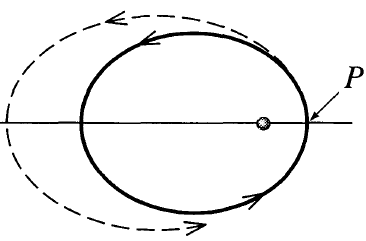
\includegraphics[width=0.85\textwidth]{Planetbevaegelse/Forward_thrust.png}
		\caption{Positivt boost således, at hastigheden øges, hvilket resulterer i et baneskift udad.}
		\label{fig:Forward_thrust}
	\end{subfigure}
	\hspace{5mm}
	\begin{subfigure}{0.45\textwidth}
		\centering
		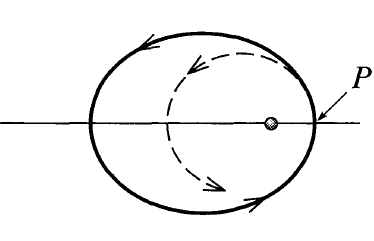
\includegraphics[width=0.85\textwidth]{Planetbevaegelse/Backward_thrust.png}
		\caption{Negativt boost således, at hastigheden sænkes, hvorved der foretages et baneskift indad.}
		\label{fig:Backward_thrust}
	\end{subfigure}
	\caption{Et objekts oprindelige bane er angivet med en streg, mens dets nye bane efter baneskift er vist med en stiplet linje. Baneskiftet foretages her i punktet $P$, hvilket kaldes periapsis, hvor punktet, der ligger lige modsat $P$ på den vandrette akse, kaldes apoapsis. (Kilde: \textit{Classical Mechanics}, John R. Taylor, figur 8.12.)}
	\label{fig:Boost_Forward_Backward}
\end{figure}

Først skal det lige fastsættes, hvad der menes med periapsis. Periapsis er det punkt på en bane, hvor der er mindst afstand mellem de to indgående objekter, hvilket i figur \ref{fig:Boost_Forward_Backward} er angivet med et $P$. Ligeledes findes et navn for det punkt på en bane, hvor der er størst afstand mellem de to indgående objekter, hvilket er apoapsis, og denne kan på figur \ref{fig:Boost_Forward_Backward} ses som liggende lige modsat $P$ på den vandrette akse.\footnote{Periapsis og apoapsis er de generelle betegnelser for disse punkter. For bestemte andre situationer findes også andre navne for disse punkter: For en bane omkring Solen benævnes periapsis og apoapsis henholdsvis perihelium og aphelium, og for en bane omkring Jorden benævnes disse henholdsvis perigæum og apogæum.}

\noindent
Scenariet, som betragtes nu, er en satellit, der foretager et baneskift, ved at affyre sine raketter enten fremad eller bagud tangentielt til dens bane, idet den befinder sig i periapsis, $\phi_0$. Koordinatsystemet for dette vælges således, at dets $x$-akse går gennem periapsis, hvor afstanden mellem Jorden og satellitten skal være kortest. Dette sker når argumentet til cosinus, $\phi_0-\delta_1$, er nul, da $\cos(0)=1$. Idet det vides, at $\phi_0$ er, når satellitten befinder sig i periapsis, og koordinatsystemets $x$-akse går gennem periapsis, da vil $\phi_0 = 0$, hvorfor $\delta_1 = 0$. Grundet at raketterne affyres i den tangentelle retning, vil satellittens retning ikke ændre sig under boostet, hvorfor den nye bane også vil have periapsis\footnote{Det er også muligt, at dette punkt kan være apoapsis, hvilket vil vise sig til sidst i afsnittet, så den mest præcise beskrivelse her ville være at sige, at den nye bane vil have apsis (et af yderpunkterne) i første banes periapsis, hvorfor $\delta = 0 \vee \delta = \pi$, men forskellen på disse er, om $\cos(\phi_0-\delta) = 1 \vee \cos(\phi_0-\delta) = -1$.} i $\phi_0$, og det derfor også må gælde, at $\delta_2 = 0$. På denne måde kan ligning \eqref{eq:r1(phi0)=r2(phi0)} reduceres til
\begin{align} \label{eq:Reduceret_r1(phi0)=r2(phi0)}
	\frac{c_1}{1+\epsilon_1} &= \frac{c_2}{1+\epsilon_2} \: .
\end{align}

\noindent
Der inføres nu en boostfaktor $\lambda$, som er svarende til forholdet mellem hastigheden efter, $v_2$, og før boostet, $v_1$,
\begin{align} \label{eq:Baneskift_boostfaktor}
	\lambda &= \frac{v_2}{v_1} \: .
\end{align}
Idet $\lambda > 1$ vil boostet være fremadrettet (positivt), da $v_2 > v_1$. For $0 < \lambda < 1$ vil boostet være tilbagerettet (negativt), da $v_2 < v_1$.

\noindent
Der laves nu to antagelser: For det første antages det, at satelittens masseændring grundet boostet er så lille, at den er negligibel, således at den reducerede masse $\mu$ er konstant før og efter boostet. For det andet antages det, at boostet foregår øjeblikkeligt, hvorfor satelitten er i samme punkt, $\phi_0$, før og efter boostet. Ud fra dette, og med viden om, at impulsmomentet er proportionelt med hastigheden, vil følgende gøre sig gældende:
\begin{align}
	\ell_2 &= \lambda \ell_1 \: ,
\end{align}
og da $c$ er proportional med $\ell^2$ fås følgende:
\begin{align} \label{eq:Baneskift_c2}
	c_2 &= \lambda^2 c_1 \: .
\end{align}
Indsættes dette i ligning \eqref{eq:Reduceret_r1(phi0)=r2(phi0)} og isoleres excentriciteten af bane 2, $\epsilon_2$, fås
\begin{align} \label{eq:Baneskift_epsilon2}
	\epsilon_2 &= \lambda^2\epsilon_1+(\lambda^2-1) \: .
\end{align}
%
Fra ligning \eqref{eq:Baneskift_epsilon2} kan det ses, at boostes satelitten positivt, $\lambda > 1$, vil den nye bane have en excentricetet større end den første bane, $\epsilon_2 > \epsilon_1$. De to baner vil altså have samme periapsis, men satelitten vil i den nye bane komme længere væk fra Jorden, se figur \ref{fig:Forward_thrust}. Ved en stor nok $\lambda$ vil excentriciteten af den nye bane blive større end $1$, hvilket er svarende til en hyperbolsk bane, hvilken er åben, hvorfor satellitten kan undslippe fra Jorden. \\
Hvis i stedet satellitten boostes negativt, således at $\lambda < 1$, vil den nye banes excentricitet være mindre end den første banes, $\epsilon_2 < \epsilon_1$, hvorfor den nye bane vil ligge indenfor den første bane, men de to baner vil stadig have samme periapsis. \\
Mindskes $\lambda$ nås et punkt, hvor $\epsilon_2 = 0$, og her kommer satelitten i en cirkulær bane omkring Jorden. Mindskes $\lambda$ fortsat opnås en negativ excentricitet, hvilket giver fin mening, når det indsættes i formlen for afstanden mellem to objekter, hvor det ene er i banebevægelse om det andet, ligning \eqref{eq:Generel_formel_r(phi)}, der så ser ud på følgende måde
\begin{align}
	r(\phi) &= \frac{c}{1-\epsilon\cos(\phi)} \: ,
\end{align}
hvilket er svarende til afstanden fra Jorden og til apoapsis, hvorfor periapsis i den første bane i dette tilfælde vil sammenfalde med apoapsis.